% vim: set spell spelllang=es syntax=tex :

\documentclass[11pt,a4paper,spanish]{beamer}

\usepackage[spanish]{babel}

\usepackage[utf8]{inputenc}

\usepackage{graphicx}

\usepackage{subcaption} %Para Subfigure

\usepackage{caption} %Para captions en las figuras sin prefijo

\usepackage{ccicons}

\usepackage{url}

\usepackage{babelbib}

\usepackage{textcomp}

\usepackage{amsmath} %Para `aligned` en las ecuaciones.

\usepackage{styles/egyptian}

\newcommand{\aprox}{\raisebox{0.5ex}{\texttildelow}}
\newcommand{\bit}{\textbf{b}}
\newcommand{\Byte}{\textbf{B}}

\usefonttheme{serif}

\setlength{\parskip}{1.5mm}

\usetheme{Rochester}
\usecolortheme{whale}

%\usetheme{Warsaw}

\beamertemplatenavigationsymbolsempty

\setbeamertemplate{background canvas}{
    \raisebox{-0.99\paperheight}[0pt][0pt]{
        \makebox[\paperwidth]{
            \null
            \hspace{-1em}
            
\includegraphics[width=0.09\paperwidth]{logos/fai.pdf}
            \hspace{0.8\paperwidth}
            \hspace{-0.5em}
            \includegraphics[width=0.09\paperwidth]{logos/uncoma.pdf}
            }
    }
}

\defbeamertemplate{footline}{centered page number}
{
    \hspace*{\fill}
    \usebeamercolor[fg]{blue}
    \usebeamerfont{page number in head/foot}
    \insertpagenumber\,/\,\insertpresentationendpage
    \hspace*{\fill}\vskip2pt
}
\setbeamertemplate{footline}[centered page number]

\title{Representación de la información:\\
Representación de números fraccionarios y reales}
\author{}
\date{}

\begin{document}

\begin{frame}[noframenumbering]
    \maketitle
    \centering
    %\vspace{-8em}~
    %\begin{figure}
    %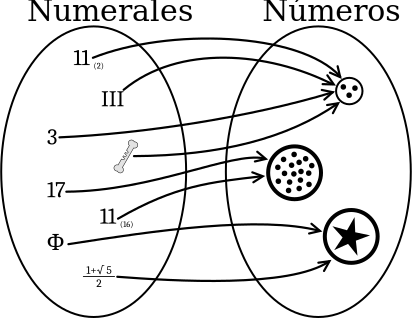
\includegraphics[height=0.65\textheight]{img/numerales.pdf}
        %\captionsetup{textfont=tiny,labelformat=empty,justification=centering}
        %\caption{}
    %\end{figure}
\end{frame}

\begin{frame}[label=temario]{Representación de datos numéricos}
\begin{itemize}
\item Fraccionarios:
    \begin{itemize}
        \item Punto Fijo.
        \item Punto Flotante.
    \end{itemize}
\end{itemize}
\end{frame}

\begin{frame}{Números fraccionarios}
\begin{itemize}
    \item Los números fraccionarios son aquellos racionales que no son
        enteros, y se escriben como una razón, fracción o cociente de dos
        enteros.
    \item Cuando se representan como decimales, la parte decimal puede ser
        finita o periódica (no finita, pero que se repite).\pause
    \item Por ejemplo $0,75$ también puede escribirse como $\frac{3}{4}$.
    \item Por ejemplo $0,\overline{3}$ también puede escribirse como
        $\frac{1}{3}$.
\end{itemize}
\end{frame}

\begin{frame}{Números irracionales}
\begin{itemize}
    \item Por otro lado, existen números reales que no son racionales (no
        existe una fracción entre enteros que los represente) pero tienen una
        representación decimal con parte entera y una parte decimal no
        periódica e infinita.\pause
    \item Por ejemplo $\sqrt{2}$ no puede escribirse como una fracción de
        enteros, pero si como\\ \pause
        $1.414213562373095048801688724209698078569671875376$\\
        $94807317667973799073247846210703885038753432764157$\\
        $27350138462309122970249248360558507372126441214970$\\
        $99935831413222665927505592755799950501152782060571$\\
        $47010955997160597027453459686201472851741864088919$\\
        $86095523292304843087143214508397626036279952514079$\\
        $89687253396546331808829640620615258352395054745750$\\
        $28775996172983557522033753185701135437460340849884$\\
        $71603868999706990048150305440277903164542478230684$\\
        $92936918621580578463111596668713013015618568987237$\\
        $23528850926486124949771542183342042856860601468247$\\
        $20771435854874155657069677653720226485447015858801$\\
        $62075847492265722600208558446652145839889394437092$\\
\end{itemize}
\end{frame}

\begin{frame}{Expresión General Extendida}

    La coma (o punto decimal) señala el lugar donde los exponentes de la base de la expresión general se
    hacen negativos.

    Sea un número $N_{(b)} = X_{k}X_{k-1}...X_{1}X_{0},X_{-1}X_{-2}...X_{-q}$, donde cada $X_{i}$ son sus
    dígitos en base $b$. Su representación en decimal $W_{(10)}$:

\begin{equation*}
\begin{aligned}
    N_{(b)} = &\sum_{i=-q}^{k} X_{i}{\times}b^{i}\\
    = &X_{k}{\times}b^{k}+X_{k-1}{\times}b^{k-1}...\\
    &X_{1}{\times}b^{1}+X_{0}{\times}b^{0}+X_{-1}{\times}b^{-1}...\\
    &X_{-q+1}{\times}b^{-q+1}+X_{-q}{\times}b^{-q}\\
    = &W_{(10)}\\
\end{aligned}
\end{equation*}
\end{frame}

\begin{frame}{Expresión General Extendida}

Ejemplos:

\begin{itemize}
    \item
        $3.14_{(10)} =
        3{\times}10^0+1{\times}10^{-1}+4{\times}10^{-2} =
        3.14_{(10)}$
    \item
        $10.01_{(10)} =
        1{\times}2^1+0{\times}2^0+0{\times}2^{-1}+1{\times}2^{-2} =
        2.25_{(10)}$
\end{itemize}
\end{frame}

\begin{frame}{Conversión de decimal a binario}
\begin{enumerate}
    \item Se separan la parte entera y la parte fraccionaria.

    \item Se convierte la parte entera a binario.

    \item La parte fraccionaria se multiplica por 2 y se toma la parte entera del resultado. Este dígito
        binario se agrega al resultado final.

    \item Se repite el paso $3$ con la nueva parte fraccionaria obtenida, hasta que ésta sea 0, o hasta
        lograr la precisión deseada.

    \item La parte entera de cada uno de los resultados del paso $4$, forman los dígitos del número en la
        base en orden de izquierda a derecha.

    \item Sumamos la parte entera a la parte fraccionaria.

\end{enumerate}
\end{frame}

\begin{frame}{Conversión de decimal a binario}

    Ejemplo: Convertir el número $3.625_{(10)}$ a base 2.

\begin{enumerate}
\item Separamos parte entera (3) y parte fraccionaria ($0.625$).

\item La parte entera se convierte a base 2 como entero sin signo (utilizando el método de la división)
    dando $11_{(2)}$.\pause

\item Expresamos la parte fraccionaria:

    \begin{enumerate}

    \item Multiplicamos la parte fraccionaria hasta obtener cero o una precisión de 5 dígitos:
        \pause
        \begin{tabular}[t]{ l r }

            $0.625{\times}2$ & = $1.25$\\\pause

            $0.25{\times}2$ & = $0.5$\\\pause

            $0.5{\times}2$ & = $1.0$\\

        \end{tabular}\pause

    \item La parte fraccionaria es $0.101$.

    \end{enumerate}\pause

    \item $3.625_{(10)}=11_{(2)} + 0.101_{(2)} = 11.101_{(2)}$

\end{enumerate}
\end{frame}

\begin{frame}{Representación de Punto Fijo \emph{(n,k)}}
\begin{itemize}
    \item Se define una cantidad fija $(n-k)$ de \textbf{bits} para la parte
        entera y $k$ \textbf{bits} para la parte fraccionaria.
    \item La computadora puede tratar aritméticamente a todos los números como
        si fueran enteros.
    \item Conversión de decimal a Punto Fijo \emph{(n,k)}:
    \begin{enumerate}
        \item Obtener la representación binaria del valor absoluto del número,
            con una precisión de \emph{k}.
        \item Expresar la parte entera y fraccionaria en la cantidad adecuada de
            \textbf{bits}. Si es necesario completar con ceros, a la izquierda
            para la parte entera, y a la derecha en la fraccionaria.
        \item Si el número es negativo, aplicar la operación de complemento a
            2.
    \end{enumerate}
\end{itemize}
\end{frame}

\begin{frame}{Conversión de decimal a Punto Fijo \emph{(n,k)}}

    Ejemplo, representar $-7,33$ en Punto fijo \emph{(8,4)}:\pause

    \begin{enumerate}
        \item $|-7,33_{(10)}| \simeq 111.0101_{(2)}$, con una precisión de
            \emph{k}.
            \pause
        \item Expresamos el número en 4\bit{} para la para la parte entera, y
            4\bit{} para la parte fraccionaria: $01110101$
            \pause
        \item Como el número es negativo, aplicamos la operación de \emph{C2}:
            $C2(01110101) = 10001011 \simeq -7,33_{(10)}$
    \end{enumerate}
\end{frame}

\begin{frame}{Representación de Punto Fijo}
\begin{itemize}
    \item Adecuada para problemas con datos de magnitudes y precisiones
        similares.
    \item Aplicada en sistemas de tiempo real.
    \item Sistemas donde es importante la velocidad de cómputo, como juegos.
    \item Sistemas empotrados o embebidos con procesadores de recursos
        limitados.
\end{itemize}
\end{frame}

\begin{frame}{Representación de fraccionarios}
\framesubtitle{Truncamiento}

    ¿Qué pasa si no es suficiente la cantidad de bits que tenemos para la parte fraccionaria?
        ¿Es realmente $1000\,1011 = -7,33_{(10)}$ con \emph{PF(8,4)}?
    \pause

    \textbf{El número almacenado será una aproximación al número original.}

    \pause

    Si quisiéramos conocer de \textbf{cuánto} es ese error, deberíamos
    calcular la diferencia entre el número que queremos representar, y el
    número representado por la computadora.

\end{frame}

\begin{frame}{Representación de fraccionarios}
\begin{itemize}
    \item ¿Qué pasa si tenemos magnitudes muy diferentes?
    \pause
    \item \small Por ejemplo, si se necesita calcular el tiempo en que la luz
        recorre una millonésima de milímetro, la fórmula relacionará la
        velocidad de la luz en $\frac{m}{s}$ (unos $300\,000\,000
        \frac{m}{s}$) con el tamaño en metros de un nanómetro ($0.000000001
        m$).
\end{itemize}
\end{frame}

\begin{frame}{Notación Científica}
\begin{itemize}
    \item Los números se expresan en una forma estandarizada que consiste de
        un coeficiente y una mantisa multiplicada por una potencia de 10: $m
        \times 10^{x}$
\pause

\begin{equation*}
\begin{aligned}
    d =& 1\times{}10^{-9}m\\
    v =& 3\times{}10^8\frac{m}{s}\\
\end{aligned}
\end{equation*}
\pause

\begin{equation*}
\begin{aligned}
    t =& \frac{d}{v} \pause =
    \frac{1\times 10^{-9}m}{3\times 10^{8}\frac{m}{s}}\\
    \pause
      =& (\frac{1}{3} \times 10^{-9-8}s)\\
    \pause
      =& 0,\overline{3}\times10^{-17}s\\
\end{aligned}
\end{equation*}

\end{itemize}
\end{frame}

\begin{frame}{Notación Científica Normalizada}
\begin{itemize}
    \item El coeficiente \textit{m} debe ser un valor mayor o igual que 1 y
        menor que 10.
    \pause
\item Ejemplo: $t = 0,\overline{3} \times 10^{-17}s\pause
    = 3,\overline{3} \times 10^{-18} s$
\end{itemize}
\end{frame}

\begin{frame}{Representación en Punto Flotante}
\framesubtitle{\emph{MiniFloat}}

Formato que utiliza la notación científica normalizada:

\begin{itemize}
    \item Se utiliza 1\bit{} para el signo.
    \item Se utilizan $n$\bit{} para el exponente en exceso a $2^{n-1}-1$.
    \item Se utilizan $k$\bit{} para la mantisa (parte decimal del número).
\end{itemize}

\end{frame}

\begin{frame}{Representación en Punto Flotante}
\framesubtitle{\emph{MiniFloat}}

Una versión didáctica del formato:

\begin{itemize}
    \item Se utiliza 1\bit{} para el signo.
    \item Se utilizan $4$\bit{} para el exponente en exceso a $7$.
    \item Se utilizan $3$\bit{} para la mantisa.
\end{itemize}

    \begin{figure}
    \centering
    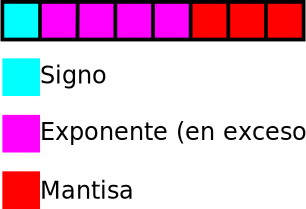
\includegraphics[width=0.5\textwidth]{img/minifloat.pdf}
    \captionsetup{labelformat=empty}
    \caption{}
    \end{figure}
\end{frame}

\begin{frame}{Conversión de decimal a punto flotante}
\begin{enumerate}
    \item Separar el signo y escribir el valor absoluto de \textit{n} en base 2.
    \item Escribir el resultado en notación científica normalizada.
    \item Expresar el exponente obtenido en el paso anterior, en exceso.
    \item El coeficiente calculado se guarda sin su parte entera en la parte
        de mantisa.
\end{enumerate}
\end{frame}

\begin{frame}{Conversión de decimal a punto flotante}

\textbf{Ejemplo:} Expresar el decimal $-5,5$ en \emph{MiniFloat}.

\begin{itemize}
    \item Necesitamos averiguar \textit{s}, \textit{e} y \textit{m}.
    \pause
    \item \textit{n} es negativo, luego $s = 1$. \pause
    \item El valor absoluto en binario es: $101,1$. \pause
    \item Normalizado: $1,011 \times 2^2$  por lo que la mantisa es $m=011$.
        \pause
    \item El exponente se representa en exceso a 7: $e = 2 + 7 = 9 = 1001_{2}$
        \pause
    \item Resultado Final: $1100\,1011$. En hexadecimal \textbf{CB}.
\end{itemize}
\end{frame}

\begin{frame}{Conversión de punto flotante a decimal}

\textbf{Ejemplo:} ¿Qué número esta representado en el \emph{MiniFloat}
    \textbf{5C}?

\begin{itemize}
    \item Necesitamos averiguar \textit{s}, \textit{e} y \textit{m}.
    \pause
    \item Convertimos el hexadecimal a binario: $\mathtt{5C}_{(16)} =
        0101\,1100$. \pause
    \item Recuperando los valores:$s = 0$, $e = 1011_{(2)} = 11_{(10)}$,
        $m = 0.100$. \pause
    \item Remplazamos los valores en la siguiente formula:
    \begin{equation*}
    \begin{aligned}
        N &= (-1)^{s} \times (1+m)_{(2)}\times 2^{(e-7)}\\
        \pause
          &= (-1)^{0} \times (1+0.100)_{(2)}\times 2^{(11_{(10)}-7)}\\
        \pause
          &= (-1)^{0} \times (1.100)_{(2)}\times 2^{(4_{(10)})}\\
        \pause
          &= 1 \times (11000.0)_{(2)}\\
        \pause
          &= 1 \times 24_{(10)} = 24_{(10)}
    \end{aligned}
    \end{equation*}
\end{itemize}
\end{frame}

\begin{frame}{Representación en Punto Flotante}
\framesubtitle{Estándar IEEE 754}
\begin{itemize}
    \item Precisión simple: 1\bit{} de signo, 8\bit{} para el exponente, y
        23\bit{} para la mantisa.
    \item Precisión doble: 1\bit{} de signo, 11\bit{} para el exponente, y
        52\bit{} para la mantisa.
\end{itemize} \pause

A pesar del incremento en la precisión, aun puede causar problemas: ¿Cuánto
    es $0.2 + 0.3$? (ver en la consola con \texttt{python3})

\end{frame}

\againframe{temario}

\begin{frame}
    \title{¿Consultas?}
    \maketitle
\end{frame}

\newcounter{lastPage}
\setcounter{lastPage}{\number\value{page}}

\setcounter{page}{\number\value{lastPage}}

\end{document}
